% LaTeX Article Template - using defaults
\documentclass[12pt]{article}
\usepackage{amsmath}
\usepackage{amssymb}
\usepackage{amsfonts}
\usepackage{amsthm}
\usepackage{mathrsfs}
\usepackage{graphicx}
\usepackage{subcaption}

\pdfpagewidth 8.5in
\pdfpageheight 11in

\usepackage[final]{showkeys}


% Set left margin - The default is 1 inch, so the following 
% command sets a 1.25-inch left margin.
\setlength{\oddsidemargin}{0.25in}

% Set width of the text - What is left will be the right margin.
% In this case, right margin is 8.5in - 1.25in - 6in = 1.25in.
\setlength{\textwidth}{6in}

% Set top margin - The default is 1 inch, so the following 
% command sets a 0.75-inch top margin.
\setlength{\topmargin}{-0.25in}

% Set height of the text - What is left will be the bottom margin.
% In this case, bottom margin is 11in - 0.75in - 9.5in = 0.75in
\setlength{\textheight}{8in}

\theoremstyle{definition}
\newtheorem{definition}{Definition}[section]


% Set the beginning of a LaTeX document
\begin{document}

\title{Generative Models}         % Enter your title between curly braces
\author{Ananya Kumar}        % Enter your name between curly braces
\date{\today}          % Enter your date or \today between curly braces
\maketitle

Suppose we have $T$ topics in $d$ dimensional space. We assume that no 3 topics are collinear. We repeatedly pick a random pair of topics $T_1$ and $T_2$. Each pair is picked with equal probability. Then we pick a uniformly random data point in the line segment connecting $T_1$ and $T_2$. We repeat this process $m$ times to generate $m$ data points.

\begin{figure}[!htb]
\centering
\begin{subfigure}[b]{.35\linewidth}
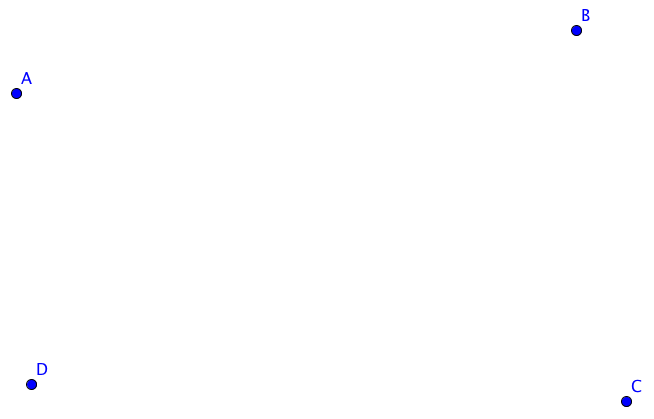
\includegraphics[width=\linewidth]{4_topics}
\caption{Start with 4 topics}\label{fig:mouse}
\end{subfigure}\hspace{20 mm}
\begin{subfigure}[b]{.35\linewidth}
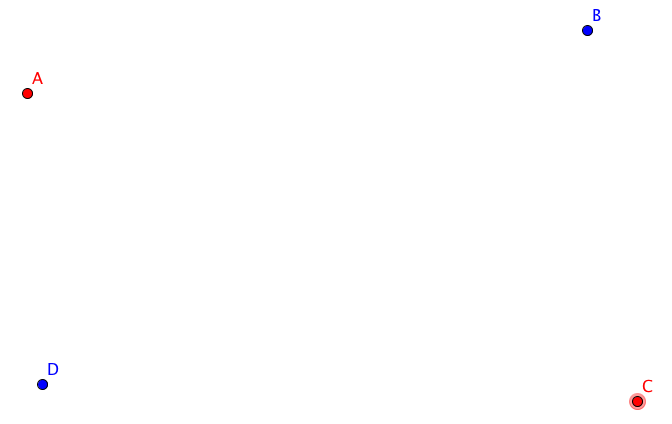
\includegraphics[width=\linewidth]{select_2_topics}
\caption{Choose 2 random topics}\label{fig:gull}
\end{subfigure}

\begin{subfigure}[b]{.35\linewidth}
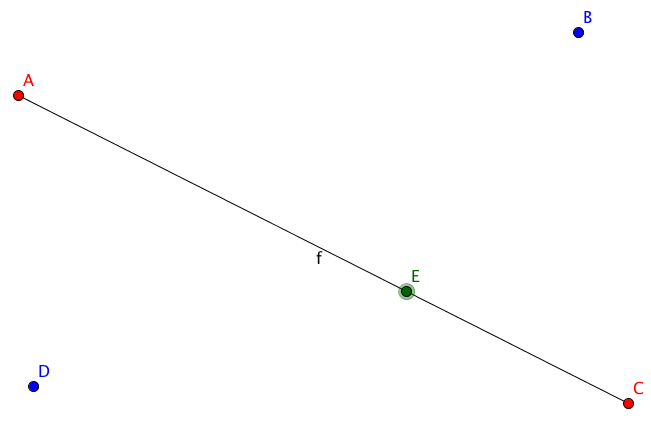
\includegraphics[width=\linewidth]{select_point_on_line}
\caption{Pick point in the middle}\label{fig:tiger}
\end{subfigure}\hspace{20 mm}
\begin{subfigure}[b]{.35\linewidth}
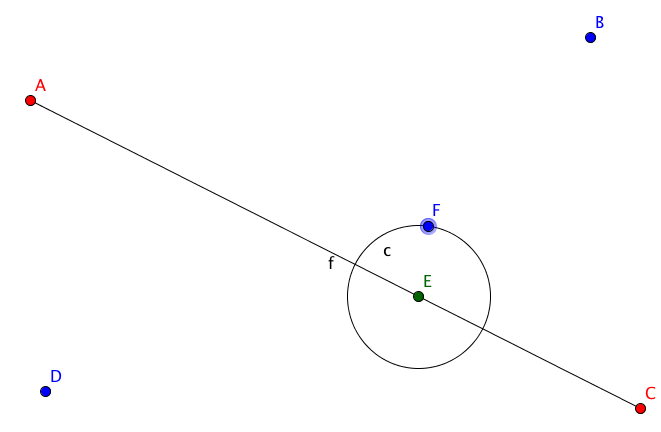
\includegraphics[width=\linewidth]{perturbed_data_point}
\caption{Pick data point in circle}\label{fig:tiger}
\end{subfigure}
\caption{Illustration of uniform noise case of generating points}
\label{fig:animals}
\end{figure}

In the noisy case, we perturb the generated data points. In the uniform noise case, the data points are perturbed so that they are uniformly random in a sphere of radius $\delta$ centered around the original location of the data point. We can also relax the distributional assumptions on how the data is generated, consider different noise models, or consider $k$-sparsity models where data points are generated from $k$ topics.



\section{Goals}

There are a few possible goals:

\begin{enumerate}
\item In the noiseless case, retrieve all T topics, exactly. Assuming we generated $\Omega(T^2\log{T})$ data points, we have a polynomial time algorithm. The probability of failure decreases exponentially with the constant factor. As an example, if we have around 50 topics, about 100,000 points are sufficient for a 99\% probability of recovering all topics. Can we recover the topics with fewer points?

\item In the uniform noise case, assuming we know the number of topics, can we recover all topics with error $\epsilon$? We probably need additional conditions to make this problem tractable.

\item Instead of recovering the topics, it could be sufficient to find $O(T)$ topic proposals. We want every data point to be within $\epsilon$ from the line segment connecting some pair of topic proposals.

\end{enumerate}

\section{Noiseless Case}

Reading this section is not too important for the rest of the document. I wrote up the details in another document, but I'll recap the key ideas for completeness.
\\

If you generate $\Omega(T^2\log{T})$ data points, with high probability every pair of topics has at least 3 data points generated between them. Pick all triplets of collinear data points, and draw an (infinite) line through them. Consider all intersections between pairs of lines. Only select pairs of intersections with data points on the (finite) line segment connecting them. Remove any intersection that is not in a selected pair. Let $S$ be the set of remaining intersections.
\\

The convex hull of $S$ is the convex hull of the topics, so we have recovered the topic convex hull. To recover the remaining topics, remove all the points on the topic convex hull from $S$. Also remove any points in $S$ that lie on a segment connecting pairs of topics in the topic convex hull. Repeat the process of selecting the convex hull and removing points until we have identified all topics (removed all the data points).

\section{Densest Point Algorithm}

I'll motivate the algorithm with a simple 2D example. Suppose we have 3 topics, $T_1, T_2, T_3$, that form an equilateral triangle in 2D space with side length $1$. Suppose we generate $m$ data points through our uniform noise generation process, with noise parameter $\delta$. We choose radius $r = \epsilon/2$, assuming $\epsilon$ is much smaller than the side length of the equilateral triangle.

\begin{definition}
Given a point $p$ in 2D space, the \emph{density} around $p$ is the proportion of generated data points that are within distance $r$ of $p$.
\end{definition}

In this case, the expected density is maximized close to the 3 topics. If $p$ is a point on the segment connecting $T_1$ and $T_2$, that is distance $r$ away from $T_1$, the density is $3r/3 = r$. If $p$ is a point on the segment connecting $T_1$ and $T_2$, that is distance $> 2r = \epsilon$ away from $T_1$ and $T_2$, the density is $\leq 2r/3$.
\\

We want a theorem that says that if $m$ is large enough, with high probability the actual density is highest near the topics. The VC dimension of a circle is 3. So we can get a uniform bound that bounds the probability that the density deviates from the expected density at any point by more than $r/3$. We can choose $m$ such that this probability is very low. Then, if we have $m$ points, with high probability we can locate the topics with error $\epsilon$ by finding the highest density point. This can be done in time polynomial in $m$.
\\

Inspired by this success, we propose the following, not yet fully precise algorithm, to recover the topics. Assume that we have generated $m$ data points, for some large $m$. We pick the data point $p$ with the highest density (as defined above, for some pre-defined $r$). $p$ is our estimate for one of the topics, in that it should be within $\epsilon$ from some topic. We then remove all the data points within distance $r'$ (for some pre-defined $r'$) of $p$. We continue the process until we recover all $T$ topics.
\\

For this particular approach, a few important tasks remain:
\begin{enumerate}
\item This algorithm does not always work efficiently. We need to impose some additional constraints. For example, if we have 3 topics that are almost collinear, then we need to generate many data points to recover the topics. What constraints does the algorithm depend on?
\item Consider the case where we have many topics, and draw the segments connecting all pairs of topics. Some of the segments intersect, and the expected density at the intersection points may be high. Does the algorithm still work in these cases, or do we need additional constraints?
\item $r$ and $r'$ might depend on constraints specific to the problem. We need to choose suitable constants for $r$ and $r'$ and complete the analysis.
\item Intuitively this algorithm could work for $k$-sparsity versions of the problem, where we generate data points from combinations of $k$ topics. It could work for other noise distributions (e.g. Gaussian) as well. This would be significant, so we could examine this case.
\end{enumerate}

% We recommend abbrvnat bibliography style.

\bibliographystyle{alpha}

% The bibliography should be embedded for final submission.

\bibliography{references}


\end{document}